\documentclass[12pt,letterpaper]{article} % twocolumn

\usepackage[left=0.8in, right=0.8in, bottom=1in, top=1in]{geometry}
\usepackage{expl3}
\usepackage[dvipsnames,table]{xcolor} % table arg for coloring table cells
\usepackage{titling}  % Customizing \maketitle

\RequirePackage{hyperref}
% Color hyperlinks dark blue by default.
\hypersetup{
    colorlinks=true,
    linkcolor=MidnightBlue,
    citecolor=MidnightBlue,
    urlcolor=MidnightBlue,
}

% Set font.
\usepackage{newtxmath}
\usepackage{fontspec}
\setmainfont{Times New Roman}
\setsansfont{Latin Modern Sans}
\setmonofont{Inconsolata}
% Bibliography.
\usepackage[backend=bibtex,style=ieee]{biblatex} % backend=bibtex
\addbibresource{EECE5639_Project_Report_McGuire_Schubert_Yeh.bib}

\usepackage{lipsum}
\usepackage[pagestyles]{titlesec}
\titlespacing{\section}
{0pc}{8pt}{4pt}[0pc] % left before after right

\titleformat{\section}[block]
{\centering\large\bfseries}
{\thesection.}
{1ex minus .1ex}
{\MakeUppercase}

\usepackage{siunitx}
\usepackage{graphicx}
\usepackage{tabularx}
\usepackage{booktabs}
\usepackage{caption}
\usepackage{subcaption}
\usepackage{float}
\captionsetup[table]{labelfont=bf}
\captionsetup[figure]{labelfont=bf}
\captionsetup[lstlisting]{labelfont=bf}

%%%%%%%%%%%%%%%%%%%%%%%%%%%%%%%%%%%%%%%%%%%%%%%%%%%%%%%%%%%%%%%%%%%%%%%%
% Tweak \maketile layout
%%%%%%%%%%%%%%%%%%%%%%%%%%%%%%%%%%%%%%%%%%%%%%%%%%%%%%%%%%%%%%%%%%%%%%%%
%\setlength{\droptitle}{-0.75in}

\DeclareDocumentCommand{\FancyEmail}{ m }{%
    \colorlet{@savecolor}{.}%
    \href{mailto:#1}{\color{@savecolor}\ttfamily{}#1}%
}
\title{\bfseries{} Quantitative Evaluation of a 3D Reconstruction Algorithm}
\author{
%    \itshape{}
    Nathan McGuire \\ \FancyEmail{mcguire.n@northeastern.edu} \and
%    \itshape{}
    Brian Schubert \\ \FancyEmail{schubert.b@northeastern.edu}\and
%    \itshape{}
    Alex Yeh \\ \FancyEmail{yeh.al@northeastern.edu}
}
\date{April 24th, 2024}

\renewcommand{\baselinestretch}{1.5}
\begin{document}
\maketitle
\vfill
\begin{abstract}
    We implement an end-to-end 3D reconstruction system and a suite of tests for quantifying its performance. The reconstruction system ingests a series of 2D images of an object and generates a representative mesh of the object in 3D space. We follow the development in \cite{9229407} to design this system. The core algorithm performs feature point extraction and triangulation to estimate 3D point clouds, from which the final mesh is reconstructed.  Furthermore, we have created a test system to generate synthetic images from 3D models.  The reconstructed meshes can be compared against the initial meshes to determine overall system performance.
\end{abstract}
\clearpage
\tableofcontents
\clearpage



\section{Introduction}
3D reconstruction is a procedure where many 2D images of a single object, taken from different poses, are used to determine the 3D geometry of the object.  Measuring the 3D geometry of objects is widely applicable, with applications ranging from planetary exploration, self-driving cars, virtual reality, and medical devices.  Using cameras for this task, instead of a sensor that can directly measure the 3D geometry, is advantageous because of the low cost of cameras and the fact that they are already widely deployed on existing systems.

It is not possible to directly compute 3D geometry from a single camera image.  Cameras measure the intensity and direction of incoming light, but not the distance to the source.  As such, at least two camera images of the same point are needed to calculate the 3D position of that point.  A simple 3D reconstruction pipeline has 3 major steps: feature extraction, feature matching, and triangulation.  Feature extraction attempts to find a large number of distinctive points in each image, feature matching attempts to pair up these points across multiple images, and triangulation uses these matches, a model of how light enters the camera, and a model of where the images were taken from to solve for the position of the points.  If the camera poses are not known, a sufficiently large number of point matches also enables the relative camera pose to be determined.  In this case, because there is no prior information about the geometry of the object or camera poses, it is not possible to determine the scale of the object, only the relative geometry of the object and camera.

A variety of factors limit the performance of real-world reconstruction systems.  Because triangulation of feature pairs relies on a model of what direction in 3D space a given pixel in image space maps to, inaccuracies in the camera model directly propagate into inaccuracies in the position of reconstructed points.  The camera model is typically determined empirically for an individual camera, since tiny variations caused by assembly can have significant impacts.  Furthermore, even a well calibrated camera will experience image noise, as camera sensors are electronic devices and are susceptible to a variety of noise sources.  This results in inaccurate pixel intensity values, which results in less feature locations.  Furthermore, since the magnitude of the noise is not constant between successive images, image noise results in differences in the feature description of a given feature in successive images, and thus less accurate feature matching.

\section{Methods}
We chose to use synthetic data to evaluate our reconstruction algorithm. This provides us with a known ground-truth mesh to compare against, and allows us to avoid pitfalls inherent in using real data, like poorly calibrated cameras.  Our image generation system is built around the pyrender library \cite{pyrender}, which is itself a python wrapper around OpenGL.  OpenGL is a widely used graphics library which handles rendering of 2D and 3D scenes.  It allows rendering of textured surfaces with a variety of realistic lighting and material effects.  Our image data generation system renders a scene constructed from a library of 3D models we’ve put together as test elements.  Individual models we used include pyrender example models of a drill and soda bottle, as well as freely accessible 3d models of coral of varying fidelity.  Rendering known 3D models ensures that the images are generated in a repeatable, consistent manner, and allows us to control for variables like the camera intrinsic parameters.  We can tune the complexity of the reconstruction by adding more or more complex 3D models to the scene and we can quantify the robustness of the reconstruction algorithm by manually adding noise to the generated images.  Generating images this way also gives us direct access to the 3D geometry used to create the images, which is crucial for evaluating the accuracy of the resulting reconstruction.

Feature extraction is performed via the OpponentSIFT algorithm \cite{5204091}.  SIFT is a feature extractor that detects distinct points using the difference of gaussians across a range of image scales, then describes the feature using the orientation of the local gradient around that point.  Because SIFT searches through the scale-space and pixel space it is invariant to feature scale changes across images.  This is useful for reconstruction, as camera motion is likely to cause changes in object scale.  Opponent SIFT is an extension to SIFT that transforms the image from a RGB colorspace to an opponent color space. The opponent color space uses three dimensions (white-black, red-green, yellow-blue). Intensity is encoded directly into one channel while the other two channels encode only color. This makes the resulting feature detections more robust with respect to illumination changes compared to traditional SIFT methods. Traditional SIFT descriptors are calculated for each opponent color space channel and flattened to form one large descriptor for each feature point.

Feature Matching is performed using brute force matching between pairs of images. For every feature in one image, the best and second best matching features in the second image are found, ranked by the L2 distance between the descriptor vectors. A ratio test is applied to filter out possibly ambiguous matches by only keeping matches if the distance to the best match divided by the distance to the second match is less than 0.8.  Outliers are further filtered using a RANSAC method on all matches between two images. OpenCV internally uses a 7-point algorithm to estimate a fundamental matrix for each RANSAC sample, and points matches are evaluated on how well they fit the epipolar geometry.

For the remaining point matches, the algebraic solution is used to recover 3D points. For a pair of features in two images, the coordinates of the features in image space are transformed into rays in camera coordinates using the known camera intrinsics. Due to the discrete nature of pixels, the rays do not intersect perfectly. Therefore, these rays are all converted into the first camera’s coordinate frame and the direction of the skew segment between these rays is calculated using their cross product. A linear system of equations is set up to calculate the lengths of the two rays and skew segment. As a final way to filter out poorly matched points, if the skew segment length is too large, the point is ignored. This is evaluated by comparing the skew segment length divided by the L2 norm of the three lengths against an empirically determined threshold of $\num{1e-2}$. If the skew segment length is not too large, the midpoint of the skew segment is taken as the triangulated point and converted into the world coordinate frame.  This process is repeated for every feature match to create the point cloud.

Once we have a point cloud, we need to reconstruct a mesh and compare against the ground truth.  A mesh is parameterized by a list of points and a list of triangular faces spanning those points.  Furthermore, the mesh needs to be closed so that we can perform comparisons against the ground truth mesh.  Though a mesh with holes is useful for a variety of reconstruction applications, the comparisons we have chosen as the baseline require the ability to compute the volume of the mesh.  There are a variety of approaches to solve this, and the current best that we have tested is Poisson Surface Reconstruction \cite{10.5555/1281957.1281965}.  This algorithm attempts to solve an optimization problem to create a smooth surface that minimizes the deviation from the point cloud.  Importantly, all the object reconstruction algorithms we tested assume that the entire point cloud belongs to a single object. As we might be imaging multiple objects, we implemented a point cloud clustering algorithm to segment the cloud by selecting continuous, dense areas.  Once we have reconstructed a mesh for an object, we compute the ratio between the intersection volume and union volume of the reconstructed and ground truth meshes.

\section{Results}
To evaluate the pipeline we created reconstructions of 6 objects.  Each object was rendered from 40 views spaced evenly around the object, which were paired sequentially into 39 pairs for feature matching.  The resulting 3D points for each pair were transformed to a common frame using the known camera extrinsics to create the final point cloud.  An example of feature extraction and matching is shown in Figure~\ref{fig:feature-match}, and an example output point cloud is shown in Figure~\ref{fig:point-cloud}.

%\let\maybefbox\fbox
\let\maybefbox\relax

\begin{figure}[h!]\centering
    \hfill
    \begin{subfigure}[b]{0.45\linewidth}\centering
        \maybefbox{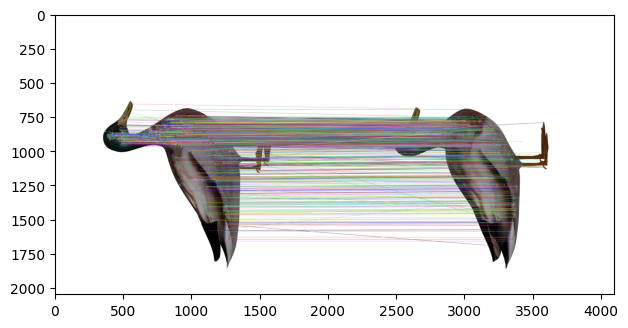
\includegraphics[width=0.9\linewidth,clip,trim={2cm 1cm 0.5cm 2cm}]{./images/duck_featurematch.png}}
        \vspace{1.5cm}
        \caption{TODO: feature match}\label{fig:feature-match}
    \end{subfigure}
    \hfill
    \begin{subfigure}[b]{0.45\linewidth}\centering
        \maybefbox{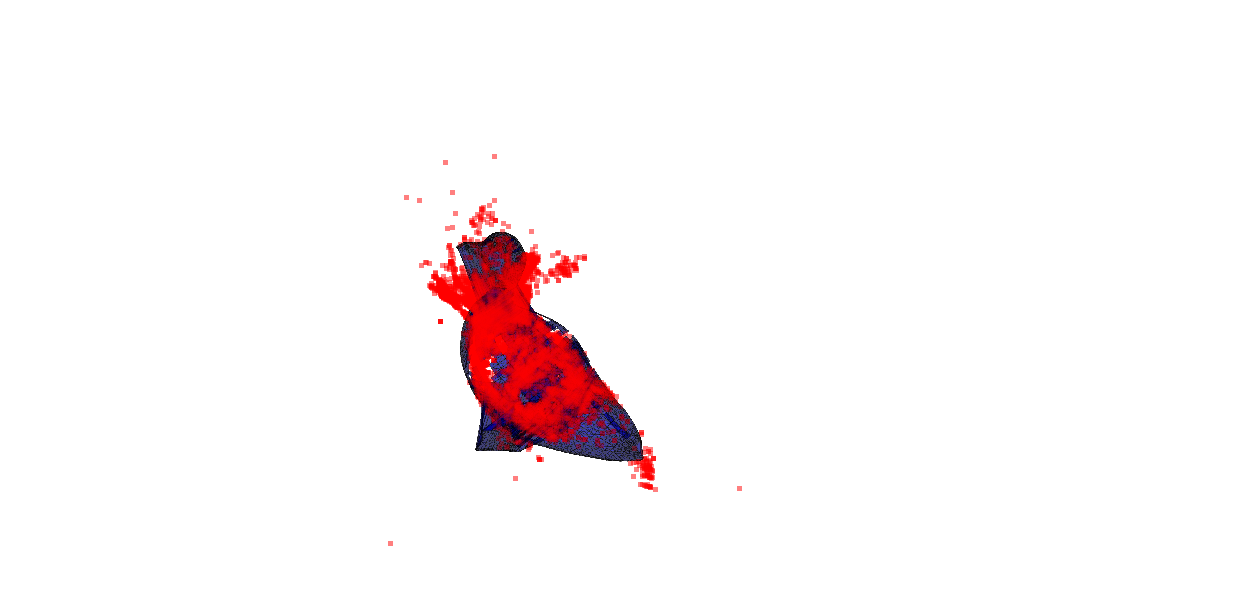
\includegraphics[width=0.9\linewidth,trim={10cm 2cm 18cm 3cm},clip]{./images/duck_points.png}}
        \caption{TODO: point cloud}\label{fig:point-cloud}
    \end{subfigure}
    \hfill
\end{figure}

The mesh reconstruction portion of the pipeline has issues.  We tested four different mesh reconstruction algorithms extensively on point clouds generated from the vertices of ground-truth meshes to verify functionality and test their robustness to added noise.  All four algorithms performed adequately against simple test data; however, none of them were sufficient to fully reconstruct a satisfactory mesh from the generated point clouds.  Failure modes ranged from simply refusing to generate any output to generating a mesh that was not ‘watertight’, meaning that it has at least one hole.  Meshes need to be watertight to have a volume, so for non-watertight meshes we are unable to calculate the intersection over union ratio.  We believe the problem is twofold: the generated point clouds have regions of lower density, and occasionally have significant artifacts.  The mesh reconstruction algorithms we tested fit into two types, those that attempt to solve an optimization problem to generate a mesh that closely matches the point cloud, and those that directly use the point cloud as vertices and attempt to solve for connections through various heuristics.  The optimization based solvers would generally fail to provide any meaningful output; we believe this was because they were not robust to the small number of large outlier points.  The heuristic based approaches likely failed for the other reason, as the heuristics they used relied on user-provided, spatial scale parameters.  Because they were essentially looking for vertex connections at specific scales, they were not robust to point clouds with sparser areas, and left gaps in the resulting mesh.

As a workaround, the intersection over union ratio of the convex hulls of the ground truth and the reconstructed mesh is shown in Table~\ref{tab:iou}.  Figures~\ref{fig:reconstruct-a} to~\ref{fig:reconstruct-e} show actual mesh reconstructions in red and the ground truth meshes used to create them in blue.

\begin{figure}[p]\centering
    \vspace{-5mm}
    \hfill
    \begin{subfigure}[b]{0.42\linewidth}\centering
        \maybefbox{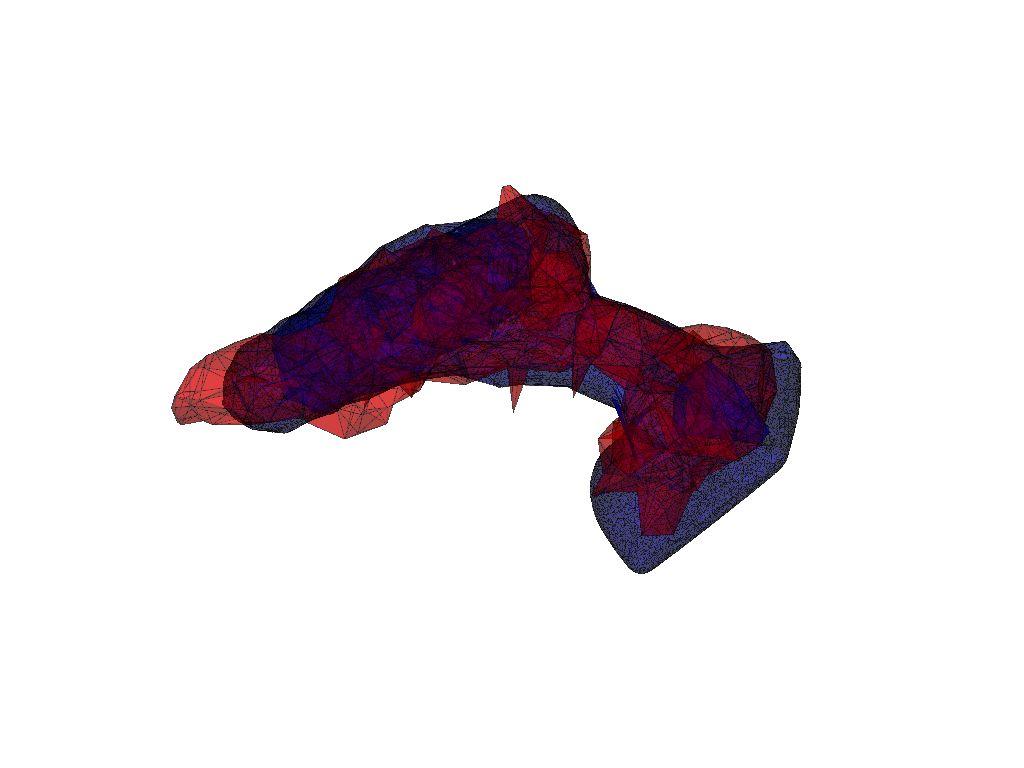
\includegraphics[width=\linewidth,trim={5cm 5cm 6cm 4cm},clip]{./images/drill_mesh_0p7288.png}}
        \caption{\texttt{drill}.}\label{fig:reconstruct-a}
    \end{subfigure}
    \hfill
    \begin{subfigure}[b]{0.42\linewidth}\centering
        \maybefbox{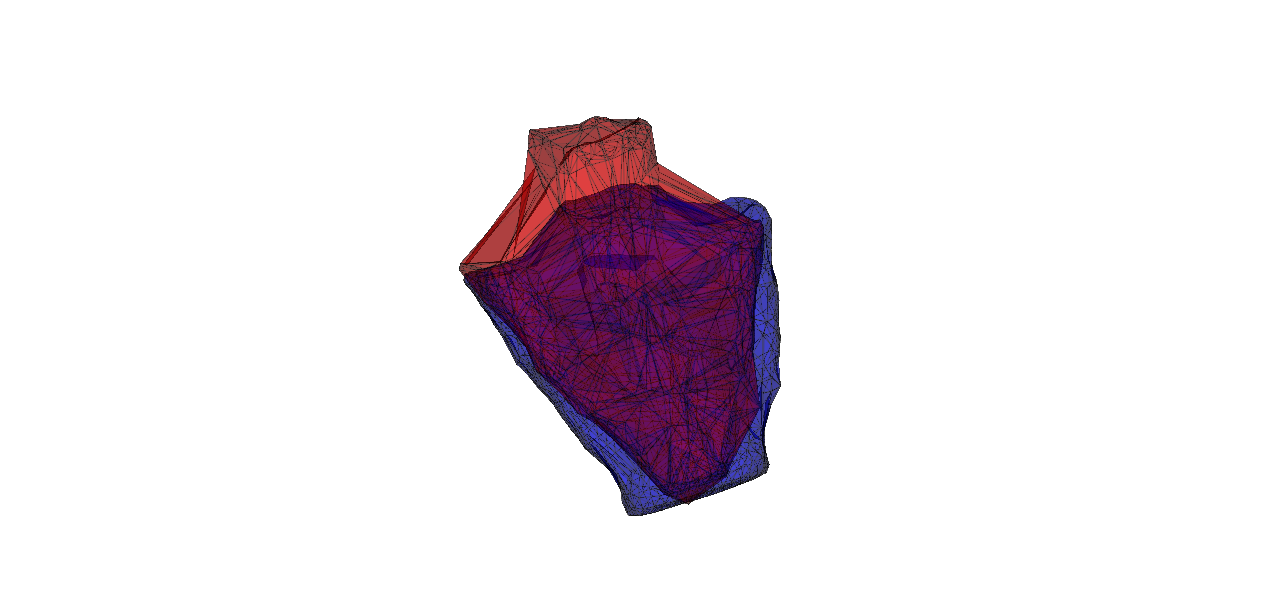
\includegraphics[width=\linewidth,trim={12cm 2cm 12cm 3cm},clip]{./images/coral4_overlap.png}}
        \caption{\texttt{coral}.}
    \end{subfigure}
    \hfill
    \\
    \hfill
    \begin{subfigure}[b]{0.42\linewidth}\centering
        \maybefbox{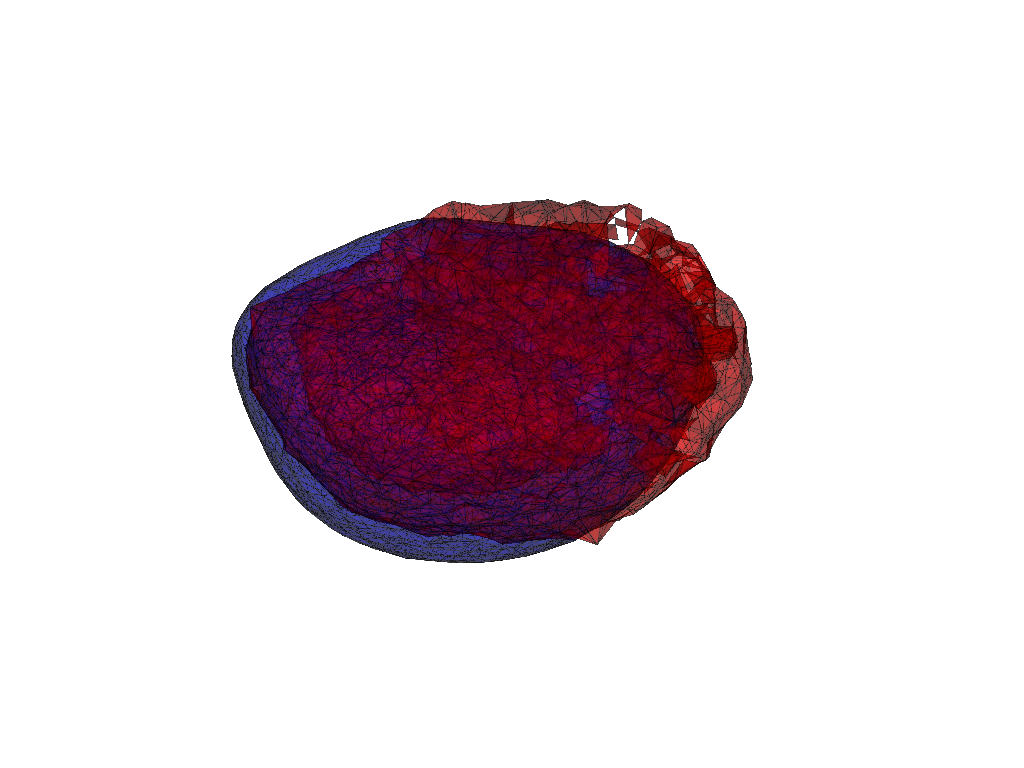
\includegraphics[width=\linewidth,trim={6cm 5cm 7cm 4cm},clip]{./images/braincoral_mesh.png}}
        \caption{\texttt{braincoral}.}
    \end{subfigure}
    \hfill
    \begin{subfigure}[b]{0.42\linewidth}\centering
        \maybefbox{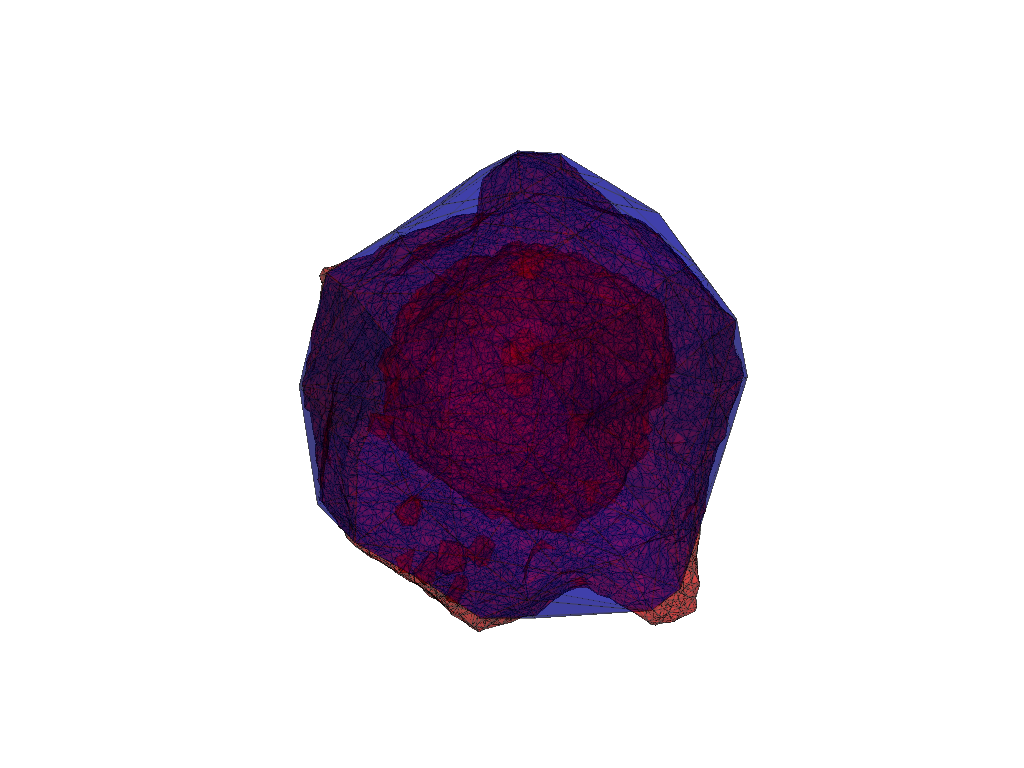
\includegraphics[width=\linewidth,trim={8cm 4cm 6cm 4cm},clip]{./images/rock_1_mesh_0p908654_2.png}}
        \caption{\texttt{rock}.}
    \end{subfigure}
    \hfill
    \\
    \hspace{0pt}
    \hfill
    \begin{subfigure}[b]{0.35\linewidth}\centering
       \maybefbox{ 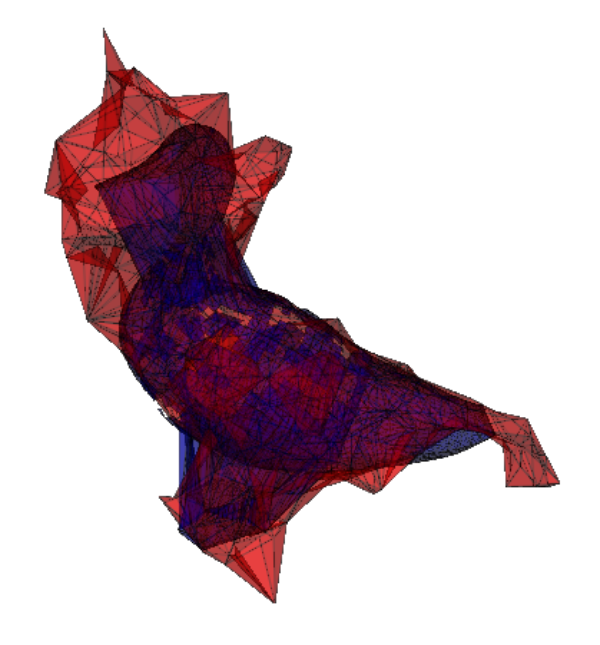
\includegraphics[width=\linewidth]{./images/duck_2.png}}
        \caption{\texttt{duck}.}\label{fig:reconstruct-e}
    \end{subfigure}
    \hfill\hspace{0pt}
    \caption{Comparison of triangulated points (red) and mesh from ground truth points (blue).}\label{fig:reconstructed-mesh}
\end{figure}

%
%\nocite{9229407}
%\nocite{DVN/CU4UXG_2021}
%\nocite{Olsson}
%\nocite{shrestha2022real}



\begin{table}\centering
    \def\arraystretch{1.2}
    \caption{Intersection-over-union ratios of reconstructed mesh convex hulls.}\label{tab:iou}
    \begin{tabularx}{0.9\linewidth}{
            >{\ttfamily}m{1.5cm}
            *{5}{S[table-format=1.6]}
        }
        \toprule
        Mesh ID & \multicolumn{1}{m{2.5cm}}{\centering{}Reference Volume}
        &  \multicolumn{1}{m{2.5cm}}{\centering{}Reconstruction Volume}
        &  \multicolumn{1}{m{2.5cm}}{\centering{}Intersection Volume}
        &  \multicolumn{1}{m{2.5cm}}{\centering{}Union Volume}
        & IOU\\
        \midrule
        drill &0.004353 & 0.003242 & 0.002466 & 0.003610 &0.710803\\
        watermelon
        &0.167625
        &0.474492
        &0.135572
        &0.506544
        &0.267642
        \\
        rock
        &0.085119
        &0.083343
        &0.080197
        &0.088262
        &0.908721\\
        coral
        &0.265899
        &0.250872
        &0.195403
        &0.321368
        &0.608038\\
        braincoral
        &0.067472
        &0.086752
        &0.060747
        &0.093479
        &0.649842\\
        duck
        &0.452759
        &1.043153
        &0.448126
        &1.047785
        &0.427689\\
        \bottomrule
    \end{tabularx}
\end{table}

%\clearpage
\section{Conclusion}
This project has implemented a 3D reconstruction algorithm pipeline and a ground truth data generation system to test it with.  Each component of the pipeline has been successfully run in isolation; however, due to time constraints, the full pipeline is not entirely functional.  We can successfully generate images of an arbitrary scene from multiple views, extract OpponentSIFT features, match them between images, and reconstruct a point cloud from the feature matches.  The mesh reconstruction portion of the pipeline is currently unable to create watertight meshes, and as such the intersection over union comparison can not be performed directly.  We believe this is likely due to a combination of noise in the reconstructed point cloud and insufficient point cloud density in some locations.

\clearpage
%\section{References}
\printbibliography%[heading=none]

\end{document}
